
%\documentclass[manuscript]{acmart}
%\documentclass[acmsmall]{acmart}
%\settopmatter{printacmref=false}


\documentclass[
  a4paper,
  12pt,
  DIV=12,        % höherer Wert = schmalere Ränder, weniger Whitespacmi
  parskip=half,  % Absätze mit halbem Abstand statt Einzug
  headings=small % kleinere Überschriften, weniger vertikaler Abstand
]{scrartcl}

%\documentclass[a4paper,11pt]{scrartcl}
%\documentclass[a4paper,11pt]{report}
%\documentclass[a4paper,12pt]{book}
\usepackage[utf8]{inputenc}
\usepackage[german]{babel}
\usepackage[T1]{fontenc}
\usepackage{lmodern}
\usepackage{graphicx}
\usepackage{amsmath}
\usepackage{caption}
\usepackage{gensymb}
\usepackage{microtype}
\usepackage{longtable}
\usepackage{tabularx}   % Spalten, die die restliche Zeilenbreite auffüllen (X-Spalte)
\usepackage{booktabs}   % \toprule \midrule \bottomrule (in mobrob_table.tex verwendet)
\usepackage{wrapfig}    % Textumfluss um Abbildungen
\usepackage{array}
\usepackage{calc}

\usepackage[citecolor=black, colorlinks=true, linkcolor=black, urlcolor=blue]{hyperref}


%\usepackage{geometry}
\usepackage{siunitx}
%\geometry{margin=2.5cm}


\usepackage{amsthm}
\usepackage{mdframed}
\usepackage{enumitem}

\newmdtheoremenv{theorem}{Theorem}

\theoremstyle{definition}
\newmdtheoremenv{derivation}{Derivation}

\providecommand{\tightlist}{%
  \setlength{\itemsep}{0pt}\setlength{\parskip}{0pt}}

%\mdfdefinestyle{leftline}{
%    topline=false, bottomline=false, rightline=false,
%    linewidth=2pt, linecolor=gray
%}
\theoremstyle{definition}
\newmdtheoremenv[style=leftline]{myalgorithm}{Algorithm}




%\usepackage{fancyvrb}







\let\Bbbk\relax
\usepackage{amssymb}


\usepackage{yfonts}

\usepackage{kvmap}

\usepackage[
    backend=biber,
    style=alphabetic,
    sortlocale=de_DE,
    natbib=true,
    %url=false,
    doi=true,
    %eprint=false
]{biblatex}
\addbibresource{references.bib}

%\usepackage[
%    backend=biber,
%    style=alphabetic,
%    sortlocale=de_DE,
%    natbib=true,
%    %url=false,
%    doi=true,
%    %eprint=false
%]{biblatex}
%\addbibresource{Literaturrecherche-Dennis/mobrob_references.bib}

\usepackage[autostyle=true,german=quotes]{csquotes}
\usepackage{trfsigns} %fourier transform arrow
\usepackage{mathrsfs} %fourier F
\usepackage{commath}

\usepackage{pgfplots}
\pgfplotsset{compat=1.18}

\usepackage{xcolor}
\usepackage{listings}
\usepackage[european]{circuitikz}
\ctikzset{tripoles/european not symbol=ieee circle}

%\usepackage[shading]{moeptikz}
%\moeptikzset{shading=true}

%\usepackage{german,longtable}

\usepackage{xcolor}
\usepackage{color}
\usepackage{url}

\usepackage{xfrac}

\usepackage{listings}
\usepackage{verbatimbox}

\usepackage{algorithm}
\usepackage{algpseudocode}

\usepackage{multirow}
\usepackage{float}
\usepackage{pdflscape}   % einzelne Querformatseiten (im PDF gedreht)

%%%% TIKZ

\usepackage{tikz}

\usepackage{pgfplots}
\usetikzlibrary{calc,
trees,positioning,arrows,
chains,shapes.geometric,
decorations.pathreplacing,
decorations.pathmorphing,shapes,
matrix,shapes.symbols,
plotmarks}
%\tikzexternalize[prefix=figures/]

%\tikzset{%
%  block/.style    = {draw, thick, rectangle, minimum height = 3em,
%    minimum width = 3em},
%  sum/.style      = {draw, circle, node distance = 2cm}, % Adder
%  input/.style    = {coordinate}, % Input
%  output/.style   = {coordinate} % Output
%}
% Defining string as labels of certain blocks.
%\newcommand{\suma}{\Large$+$}
%\newcommand{\multa}{\Large$\times$}
%\newcommand{\inte}{$\displaystyle \int$}
%\newcommand{\derv}{\huge$\frac{d}{dt}$}

\usetikzlibrary{arrows,automata,positioning}
%\usepackage{automata}


%%% END TIKZ

\usepackage[section]{placeins}

\usepackage{textcomp}


\usepackage{listings}
\usepackage{verbatimbox}

\usepackage{bold-extra}

\usepackage{framed}

%\usepackage{fancyhdr}
%\pagestyle{fancy}
%\lhead{\leftmark}
%\chead{}
%\rhead{}
%\lfoot{}
%\cfoot{\thepage}
%\rfoot{}
%\renewcommand{\headrulewidth}{0.2pt}
%\renewcommand{\footrulewidth}{0.2pt}



\newcommand{\Z}{\mathbb{Z}}
\newcommand{\R}{\mathbb{R}}
\newcommand{\C}{\mathbb{C}}
\newcommand{\N}{\mathbb{N}}
\newcommand{\SqrtNy}{$\sqrt{\textsc{Ny}}$}
\newcommand{\conj}{\overline}
\newcommand{\Kset}{\textswab{K}}
\newcommand{\Qset}{\textswab{Q}}
\newcommand{\ceil}[1]{\left\lceil #1 \right\rceil}
\newcommand{\floor}[1]{\left\lfloor #1 \right\rfloor}
\newcommand{\sorted}[1]{\textsc{sort}\left\lbrace #1 \right\rbrace}
\newcommand{\SNRgain}{a_{SNR}}
\newcommand{\EQgain}{a_{EQ}}
\newcommand{\SIRgain}{a_{SIR}}
\newcommand{\SNIRgain}{a_{SINR}}
\newcommand{\SNR}{\textsc{SNR}}
\newcommand{\CIRgain}{a_{CIR}}
\newcommand{\CINRgain}{a_{CINR}}
\newcommand{\CNR}{\textsc{CNR}}
\newcommand{\CINR}{\textsc{CINR}}
\newcommand{\HPAModel}{ Hughes 1177H TWTA }
\newcommand{\bigO}{\mathcal{O}}
\newcommand{\CopWinCompl}{2.375377}
\newcommand{\IBO}{\textsc{IBO}}
\newcommand{\OBO}{\textsc{OBO}}
\newcommand{\spacepage}{\newpage\null\thispagestyle{empty}\newpage}
\newcommand{\satcom}{ SatCom }
\newcommand{\db}{~\text{dB}}


\definecolor{mGreen}{rgb}{0,0.6,0}
\definecolor{mGray}{rgb}{0.5,0.5,0.5}
\definecolor{mPurple}{rgb}{0.58,0,0.82}
\definecolor{backgroundColour}{rgb}{0.95,0.95,0.92}

\lstdefinestyle{CStyle}{
    backgroundcolor=\color{backgroundColour},
    commentstyle=\color{mGreen},
    keywordstyle=\color{magenta},
    numberstyle=\tiny\color{mGray},
    stringstyle=\color{mPurple},
    basicstyle=\footnotesize,
    breakatwhitespace=false,
    breaklines=true,
    captionpos=b,
    keepspaces=true,
    numbers=left,
    numbersep=5pt,
    showspaces=false,
    showstringspaces=false,
    showtabs=false,
    tabsize=2,
    language=C
}

\lstdefinelanguage{VHDL}{
  morekeywords=[1]{library,use,all,entity,is,port,in,out,end,architecture,of,begin,process,if,then,else,elsif,when,others,signal,variable,wait,for,loop},
  morecomment=[l]--,
  morestring=[b]",
  sensitive=true
}

\lstset{
  language=VHDL,
  basicstyle=\ttfamily\small,
  keywordstyle=\color{blue},
  commentstyle=\color{gray},
  stringstyle=\color{red},
  numbers=left,
  numberstyle=\tiny,
  stepnumber=1,
  numbersep=8pt,
  frame=single,
  breaklines=true,
  captionpos=b
}

\lstset{numbers=none}

%\newcounter{example}
%\renewcommand{\theexample}{\thesection.\arabic{example}}


% Default fixed font does not support bold face
\DeclareFixedFont{\ttb}{T1}{txtt}{bx}{n}{12} % for bold
\DeclareFixedFont{\ttm}{T1}{txtt}{m}{n}{12}  % for normal

% Custom colors
\usepackage{color}
\definecolor{deepblue}{rgb}{0,0,0.5}
\definecolor{deepred}{rgb}{0.6,0,0}
\definecolor{deepgreen}{rgb}{0,0.5,0}

\usepackage{listings}

% Python style for highlighting
\newcommand\pythonstyle{\lstset{
language=Python,
basicstyle=\ttm,
morekeywords={self},              % Add keywords here
keywordstyle=\ttb\color{deepblue},
emph={MyClass,__init__},          % Custom highlighting
emphstyle=\ttb\color{deepred},    % Custom highlighting style
stringstyle=\color{deepgreen},
frame=tb,                         % Any extra options here
showstringspaces=false
}}


% Python environment
\lstnewenvironment{python}[1][]
{
\pythonstyle
\lstset{#1}
}
{}

% Python for external files
\newcommand\pythonexternal[2][]{{
\pythonstyle
\lstinputlisting[#1]{#2}}}

% Python for inline
\newcommand\pythoninline[1]{{\pythonstyle\lstinline!#1!}}





\nocite{*}


\begin{document}
%\pagenumbering{roman}



\title{Coasterbot}
\subtitle{Unternehmensvorstellung}
\author{Dennis Borutta}
%\email{gereonsuch@suchdsp.com}
%\affiliation{
%  \institution{Wilhelm Büchner University of Applied Sciences}
%  \department{Computer Engineering}
%  \city{Hof}
%  \country{Germany}
%}



\begin{titlepage}
  \begin{center}
    {\large Wilhelm Büchner University of Applied Sciences} \\[0.3em]

    {\normalsize Projektseminar Master}
\vspace{5em}

    {\LARGE\bfseries Coasterbot} \\[0.5em]

    {\large Unternehmensvorstellung} \\[1em]

    {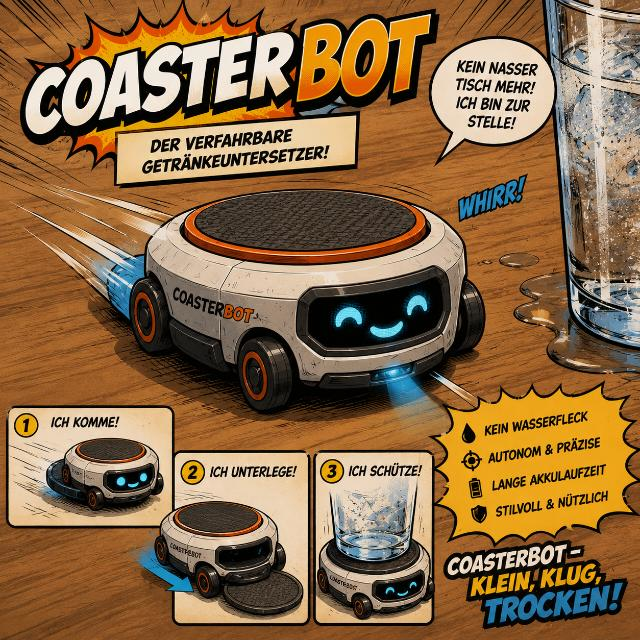
\includegraphics[width=0.38\textwidth]{coasterbot.png}} \\[1em]

\vspace{4em}

    {\normalsize
\begin{tabular}{ll}
Dennis Borutta, B. Eng & dennis.borutta@outlook.com\\
Stefan Etringer, B. Eng & mail@stefan.works\\
Gereon Such, M. Sc. & gereonsuch@gmail.com\\
\end{tabular}
    }
  \end{center}


\end{titlepage}


% einleitung preambel etc.


% Versionshistorie des Dokuments -- eigene Seite direkt nach dem Titelblatt
\section*{Versionshistorie}

\begin{tabularx}{\textwidth}{@{}clp{2.6cm}X@{}}
\toprule
\textbf{Version} & \textbf{Datum} & \textbf{Bearbeiter} & \textbf{Änderungen}\\
\midrule
1 & 19.08.2026 & Borutta & Erstfassung der Unternehmensvorstellung\\
2 & 26.08.2026 & Borutta & Erweiterung um eine Wirtschaftlichkeitsbetrachtung\\
\bottomrule
\end{tabularx}


\newpage

\tableofcontents

\newpage

\section{Unternehmensvorstellung}\label{unternehmensvorstellung}

Das Projektteam tritt als Ingenieurbüro unter dem Namen „B·E·Sondere
Lösung UG`` auf. Unser Ingenieurbüro ist darauf spezialisiert,
Prototypen und Kleinserien für Geräte und Maschinen im
Konsumentenbereich zu entwickeln und umzusetzen.

Dabei begleiten wir unsere Kunden entlang des gesamten
Entwicklungsprozesses -- von der ersten Idee über Projektierung und
Konzeption, Konstruktion und Prototypenbau bis hin zu Fertigung, Aufbau,
Erprobung und Optimierung. So entsteht aus einer ersten Produktidee eine
technisch ausgereifte und marktreife Lösung.

Sollte sich ein Produkt über die Kleinserie hinaus erfolgreich am Markt
etablieren, unterstützen wir unsere Kunden auch bei der Überführung in
größere Fertigungsstrukturen. Dabei beraten wir unter anderem beim
Aufbau geeigneter Fertigungsstrecken und sorgen dafür, dass das bereits
während der Entwicklung aufgebaute Know-how auch in der Serienproduktion
genutzt werden kann.

B·E·Sondere Lösung steht somit für eine ganzheitliche
Entwicklungsbegleitung -- von der ersten Idee bis zur
fertigungsgerechten Umsetzung. Wir sind an Ihrer Seite, um aus Ihrer
Idee nicht nur eine gute, sondern eine B·E·Sondere Lösung zu machen.

\section{Auftrag Coasterbot}\label{auftrag-coasterbot}

Der Auftrag zur Entwicklung eines Prototyps für einen Coasterbot kommt
vom Kunden „Pay With Fun GmbH``. Bei dem Kunden handelt es sich um einen
Zahlungsdienstleister, der mit kreativen Bezahlmethoden Marktanteile im
Bereich der Zahlungsdienstleistungen gewinnen konnte. Um seinen
Marktanteil weiter auszubauen, möchte er nun ein Gadget für Restaurants,
Events und Bars auf den Markt bringen, welches neben einem besonderen
Erlebnis bei der Bezahlung auch einen Mehrwert für Gastronomen bietet.

Hierdurch ist die Idee des Coasterbots entstanden. Der Coasterbot soll
folgende Mehrwerte bieten:

\begin{itemize}
\tightlist
\item
  Getränkeuntersetzer ausgeben und aufnehmen
\item
  Eine Tischoberfläche reinigen
\item
  Einen Bezahlvorgang spielerisch gestalten
\item
  Einen Bezahlvorgang beschleunigen
\end{itemize}

Die Aufgabe des Auftragnehmers „B·E·Sondere Lösung UG`` besteht bei
diesem Auftrag darin, eine technische Lösung für diese Idee zu
entwickeln. Definierte Ausbaustufen und Anforderungen sind in einem
Lasten- und Pflichtenheft festgelegt. Vom Kunden wird im Rahmen dieses
Projekts ein erster Prototyp mit minimalem Funktionsumfang gefordert.

\subsection{Finanzierung}\label{finanzierung}

Die „B·E·Sondere Lösung UG`` finanziert ihre Projekte über
Kundenaufträge. Auf Grundlage der Kundenanforderungen wird zunächst eine
Kosten- und Ressourcenplanung durchgeführt. Diese bildet die Grundlage
für die Angebotserstellung und den anschließenden Vertragsabschluss.

Die Vergütung erfolgt projektbezogen und wird in mehreren
Abschlagszahlungen entsprechend dem Projektfortschritt abgerechnet. Bei
Projektstart wird eine erste Zahlung in Höhe von 25 \% des vereinbarten
Projektpreises fällig. Nach der erfolgreichen Erstellung und Abnahme des
Umsetzungskonzepts wird eine weitere Zahlung in Höhe von 25 \% fällig.
Eine dritte Zahlung in Höhe von 25 \% erfolgt nach Auslieferung des
vereinbarten Projektergebnisses. Die verbleibenden 25 \% werden nach der
erfolgreichen Abnahme des Projektergebnisses durch den Kunden fällig.

Durch die Abrechnung nach definierten Projektmeilensteinen wird
sichergestellt, dass die Finanzierung des Projekts mit dem erbrachten
Leistungsstand fortschreitet und die „B·E·Sondere Lösung UG`` ihre
bereits erbrachten Leistungen und entstandenen Aufwendungen laufend
abrechnen kann.

\subsubsection{Wirtschaftlichkeitsbetrachtung}\label{Rentabilitaet}
Zur Beurteilung, ob sich der Auftrag für die „B·E·Sondere Lösung UG`` lohnt, wird eine Wirtschaftlichkeitsbetrachtung durchgeführt. Hierbei werden die Methodiken der statischen Investitionsrechnung angewendet. Dazu werden zunächst die Kosten und Erlöse des Projekts betrachtet. Mit diesen wird anschließend eine Gewinnvergleichsrechnung durchgeführt, um die Rentabilität des Projekts zu beurteilen. Anschließend wird ein Liquiditätsplan erstellt, um zu Erkennen wie hoch die Vorleistungen innerhalb des Projekts sind.\cite{Niemann2019Investitionsrechnung}\cite{BibEntry2026Aug}

\subsubsection{Kosten- und Erlösbetrachtung}\label{Kosten-und-Erlösbetrachtung}
Für die Kostenbetrachtung werden die bereits ermittelten Werte aus der Kostenplanung herangezogen. Hierbei wurde \textbf{Materialkosten} in Höhe von \textbf{207,00€} und ein \textbf{Stundensatz} von \textbf{89,00€/h} für die Arbeitszeit der Projektmitglieder angenommen. Hieraus ergeben sich die \textbf{Vollkosten des Projekts} in Höhe von \textbf{51.827,00€} beim Projektumfang von 580h.

Dem Gegenüber stehen die Erlöse des Projekts. Dem Auftraggeber wird ein Stundensatz von 100,00€/h in Rechnung gestellt. Hieraus ergeben sich die \textbf{Erlöse des Projekts} in Höhe von \textbf{58.000,00€}. Dazu werden die \textbf{Materialkosten} des Projekts in Höhe von \textbf{207,00€} mit einem Aufschlag von 10\% in Rechnung gestellt. Damit dem Auftraggeber Materialkosten in Höhe von \textbf{227,70€} in Rechnung gestellt. Diese aufsummiert ergeben den \textbf{Gesamterlös des Projekts} in Höhe von \textbf{58.227,70€}.

\subsubsection{Gewinnvergleichsrechnung}\label{Gewinnvergleichsrechnung}
Zur Gewinnvergleichsrechnung werden die Kosten und Erlöse des Projekts gegenübergestellt. Hierbei ergeben sich die \textbf{Gewinne des Projekts} in Höhe von \textbf{6.400,70€} wie sich aus Tabelle\ref{tab:Gewinnvergleich} ergibt.

\begin{table}[H]
\centering
\begin{tabular}{|c|c|c|c|}
\hline
\textbf{} & \textbf{Kosten} & \textbf{Erlöse} & \textbf{Gewinn} \\
\hline
\textbf{Materialkosten} &  207,00€ & 227,70€ & 20,70€ \\
\hline
\textbf{Arbeitskosten} & 51.620,00€ & 58.000,00€ & 6.380,00€ \\
\hline
\textbf{Summe} & \textbf{51.827,00€} & \textbf{58.227,70€} & \textbf{6.400,70€} \\
\hline
\end{tabular}
\caption{Gewinnvergleichsrechnung}\label{tab:Gewinnvergleich}
\end{table}


\subsubsection{Rentabilität}\label{Rentabilität}
Zur Berechnung der Rentabilität wird die Formel aus \cite{Niemann2019Investitionsrechnung} verwendet. Hierbei wird der Gewinn des Projekts durch die Kosten des Projekts geteilt und mit 100 multipliziert. Hieraus ergibt sich eine Rentabilität von \textbf{12,35\%}. Damit ist das Projekt wirtschaftlich rentabel und lohnt sich für die „B·E·Sondere Lösung UG``.

\subsubsection{Liquiditätsplanung}\label{Liquiditätsplanung}
Damit die „B·E·Sondere Lösung UG`` ihre laufenden Kosten während des Projekts decken kann, wird eine Liquiditätsplanung durchgeführt. Hierbei werden die Kosten und Erlöse des Projekts auf die einzelnen Projektmeilensteine verteilt. Dabei wird die vierteilige Zahlungsvereinbarung wir in Kapitel \ref{finanzierung} beschrieben berücksichtigt. Dabei soll erkennbar sein mit welchen Vorleistungen die „B·E·Sondere Lösung UG`` während des Projekts rechnen muss. Die Liquiditätsplanung ist in Tabelle \ref{tab:Liquiditaetsplanung} dargestellt. Die eingetragenen Werte stammen dabei aus der Kostenplanung zum Projektaufsatz. Hieraus ist zu erkennen, dass während der Umsetzungsphase an dessen Ende die Auslieferung des Prototyps steht, eine negative kumulierte Liquidität von \textbf{-1.926,21€} entsteht. Diese muss durch die „B·E·Sondere Lösung UG`` vorfinanziert werden. 

\begin{table}[H]
\centering
\small
\begin{tabular}{|l|r|r|r|r|}
\hline
\textbf{Meilenstein} & \textbf{Kosten} & \textbf{Erlöse} & \textbf{Liquidität} & \textbf{Kum. Liquidität} \\
\hline
Projektstart & 7.298,00€ & 14.556,93€ & 7.258,93€ & 7.258,93€ \\
\hline
Abnahme Konzept & 13.350,00€ & 14.556,93€ & 1.206,93€ & 8.465,86€ \\
\hline
Auslieferung Prototyp & 24.949,00€ & 14.556,93€ & -10.392,07€ & -1.926,21€ \\
\hline
Abnahme Prototyp & 6.230,00€ & 14.556,91€ & 8.326,91€ & 6.400,70€ \\
\hline
\textbf{Summe} & \textbf{51.827,00€} & \textbf{58.227,70€} & \textbf{6.400,70€} & \\
\hline
\end{tabular}
\caption{Liquiditätsplanung}\label{tab:Liquiditaetsplanung}
\end{table}

\newpage
\printbibliography[title={Literaturverzeichnis}]



\end{document}
